\documentclass[10pt]{article}

% Sprachliche Besonderheiten %%%%%%%%%%%%%
\usepackage[ngerman]{babel} % Umlaute etc.
%\usepackage[english]{babel}
\usepackage[utf8x]{inputenc} % Input encoding des Dokuments
\usepackage[T1]{fontenc} % Font encoding des Dokuments
% %%%%%%%%%%%%%%%%%%%%%%%%%%%%




% Ansprüche an mathematische und physikalische Notation %%%%%%%%%%%%%
\usepackage{amsfonts,amsmath,amsthm,amssymb} %% erweiterte Funktionalität für Formeln (Pakete der American Mathematical Society)
\usepackage[separate-uncertainty]{siunitx} %% vordefinierte Einheiten, einfaches Angeben von Einheiten (\SI{8 \pm 1}{cm}), die Unsicherheit soll mit +- abgetrennt werden, bei siuntix funktioniert babel leider nicht
\sisetup{
    range-units = single,       % \SIrange soll die Einheit nur einmal anzeigen
    list-units  = repeat,         % \SIlist soll die Einheit wiederholen
}
\sisetup{                            %% für englische Dokumente sollten diese Zeilen auskommentiert werden.
    range-phrase         = { bis },
    list-final-separator = { und },
% list-pair-separator  = { und }, % an Uni noch nicht verfügbar
}
% %%%%%%%%%%%%%%%%%%%%%%%%%%%%%%%%%%%%%%%%%%%%%%%




% Tabellen %%%%%%%%%%%%%
\usepackage{microtype} %% optimiert das typographische Erscheinungsbild
\usepackage{enumitem} %% erlaubt Listen einfacher zu formatieren (bietet nosep für kompakte Listen)
\usepackage{ctable} %% erlaubt hübsche Tabellen über mehrere Seiten, beinhaltet booktabs (\toprule, \midrule, ...)
\usepackage{xcolor} %% ermöglicht farbigen Text ({\color{red} ...})
% %%%%%%%%%%%%%%%%%%




% Bilder %%%%%%%%%%%%%%%%%%%%%%%%%%%%%%%%%%%%%%%%%%%
%% erlaubt es Bilddateien einzubinden
%% (ctable graphicx intern auch. Trotzdem ist es sinnvoll graphicx expilizt zu laden.
%%  Sonst entstehen schwehr verständliche Fehler, wenn ctable entfernt wird)
\usepackage{graphicx}
\usepackage{wrapfig}
\usepackage{floatflt}
\usepackage{float} %% ermöglicht Bilder und Tabellen am eingegebenen Ort zu platzieren ([H])
\usepackage{subfig} %% ermöglicht Unter-Bilder in einer figure-Umgebung
%%\path{{img/}} %% Grafik-Dateien werden in den folgenden Ordnern gesucht
\DeclareGraphicsExtensions{.pdf,.png,.jpg} %% Grafikdateien haben die folgenden Endungen (höchste Priorität zu erst)
% %%%%%%%%%%%%%%%%%%%%%%%%%%%%%%%%%%%%%%%%%%%%%%%




% Layout und PDFLatex %%%%%%%%%%%%%%%%%%%%%%%%%%%%%%%%%%%%%%%%%%
\usepackage{parskip}                 %% Vertikaler Abstand zwischen Absätzen, Beginn eines Absatzes nicht einrücken
% \setlength{\parskip}{0.6em}   % Vertikaler Abstand zwischen Absätzen anpassen
% \setlength{\parindent}{0em}   % Einrück-Abstand anpassen

\usepackage[                             %% Seiten-Layout einstellen  
 a4paper,
 total={16cm,26cm},                  % Breite und Höhe des Inhalt-Bereichs
 top=20mm, left=30mm,            % Ränder oben und links
 headsep=10mm,                       % Abstand des unteren Rands der Kopfzeile vom oberen Rand des Inhalts
 footskip=10mm                        % Abstand des unteren des Inhalts zum oberen Rand der Fusszeile
]{geometry}
% %%%%%%%%%%%%%%%%%%%%%%%%%%%%%%%%%%%%%%%%%%%%%%%%%%%%%%%




% Links intern/extern %%%%%%%%%%%%%%%%%%%%%%%%%%%%%%%%%%%%%%%%%%
\usepackage[                            %% Ermöglicht Links im PDF, sollte möglichst spät in der Präambel geladen werden
 pdftex,                                    % wir verwenden pdftex/pdflatex
 bookmarks=true,                      % wir wollen auch im PDF-Reader ein Inhaltsverzeichnis
 bookmarksdepth=3,                 % das Inhaltsverzeichnis soll 3 Tiefen enthalten
 colorlinks=true,                        % Linktexte sollen Farbig sein
 linkcolor=black,                        % Links innerhalb des Dokuments bleiben schwarz
 citecolor=black,                       % Links zu Quellenangaben bleiben ebenfalls schwarz
 urlcolor=blue,                          % URL-Linktexte sollen blau dargestellt werden
%  pdfborder={0 0 0}               % Links im PDF erhalten keinen Rahmen, nur nötig wenn colorlinks=false
]{hyperref}

\usepackage[english, capitalise]{cleveref} % definiert \cref: Referenzen mit korrekter Bezeichnung (z.B. "Abbildung 1"), die Nummer alleine ist weiter mittels \ref verfügbar, muss NACH 'hyperref' geladen werden
%\usepackage[german]{cleveref}
% %%%%%%%%%%%%%%%%%%%%%%%%%%%%%%%%%%%%%%%%%%%%%%%%%%%%%%




% Anderes %%%%%%%%%%%%%%%%%%%%%%%%%%%%%%%%%%%%%%%%%%
\usepackage[final]{pdfpages} %% PDF einfügen 
\usepackage[final]{showkeys} %zeige Labels im Seitenrand. Dies ist praktisch um Verweise zu kontrollieren, die Option 'final' deaktiviert die Ausgabe von showkeys
% %%%%%%%%%%%%%%%%%%%%%%%%%%%%%%%%%%%%%%%%%%%%%%%




%% Angaben für \maketitle %%%%%%%%%%%%%
\title{Programmieren einer Webseite auf der man C++-Files schreiben und ausführen kann}
\author{Nicola Krull}         
%%%%%%%%%%%%%%%%%%%%%%%%%%%%








\begin{document}
	
	\begin{titlepage}
	\begin{center}
	\huge
	\textbf{Programmieren einer Webseite auf der man C++-Files schreiben und ausführen kann}
	
	\vspace{1cm}	
	
	\LARGE
	\textbf{Nicola Krull}
	\end{center}
\end{titlepage}
	
	\tableofcontents
	\newpage
	\section{Abstract}
	\section{Einleitung}
	\pagebreak
	\section{Aufbau}
	\subsection{Design}
	
	\subsection{Software}
	Das Ziel des Projektes ist eine dynamische Webseite zu bauen. Eine dynamische Webseite ist eine Webseite bei welcher der Server mit der Webseite kommuniziert.\footnote{\label{foot:1}\href{https://blog.kompaktdesign.com/webdesign/statisch-vs-dynamisch/}{https://blog.kompaktdesign.com/webdesign/statisch-vs-dynamisch} \bigskip 30.12.2018} % Ergänzung möglich  
	Um eine dynamische Webseite zu bauen benötigt man ein Webframework, welches die Interaktionen zwischen den 			Files steueren kann. Dafür verwendete man das Webframework \textit{Express}. Es ist ein serverseitiges Webframework, welches für die Plattform \textit{Node.js} entwickelt wurde.\footnote{\label{foot:1}\href{https://de.wikipedia.org/wiki/Express.js}{https://de.wikipedia.org/wiki/Express.js} \bigskip 25.10.2018} \textit{Node.js} ist eine open-source, serverseitige Plattform, welche \textit{JavaScript} als Skriptsprache verwendet.\footnote{\label{foot:2}\href{https://de.wikipedia.org/wiki/Node.js}{https://de.wikipedia.org/wiki/Node.js} \bigskip 25.10.2018}	Wenn man eine dynamische Webseite programmiert muss man immer zwischen serverseitigen und clientseitigen Code unterscheiden. Für die serverseitigen Programme verwendet man, die Plattform \textit{Node.js} und auf der Clientenseite läuft \textit{JavaScript}, \textit{HTML} und \textit{CSS}-Code. Dabei verwendet man die Templatesprache \textit{Jade}, welche zur Generierung von \textit{HTML}-Seiten zuständig ist. Es vereinfacht nicht nur die Syntax, sondern es funktion wie anderen Programmiersprachen, somit kann man für den \textit{HTML}-Code Variabeln, If-Abfragen und for-Schleifen benützen. \footnote{\label{foot:3} \href{https://t3n.de/news/jade-638027/}{https://t3n.de/news/jade-638027/} \bigskip 25.10.2018}

\begin{floatingfigure}[r]{11cm}
    \centering
    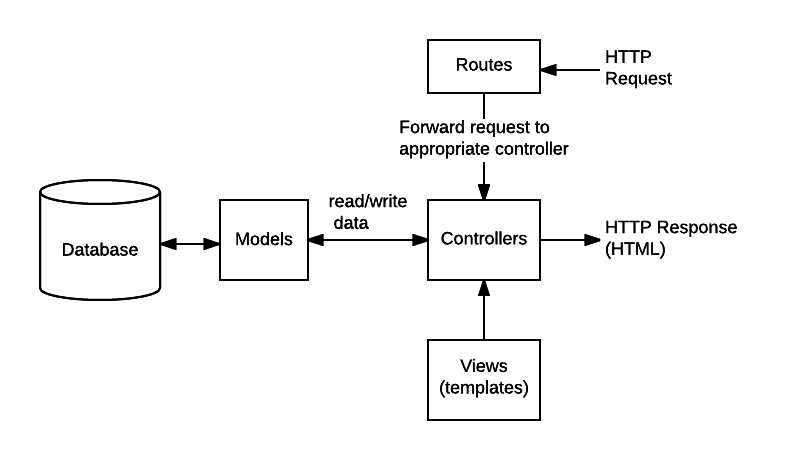
\includegraphics[width=10cm]{Bilder/MVCexpress.png}
    \caption{Express Aufbau}
    \label{fig:figlabel}
\end{floatingfigure}

\textit{Express} kann man in die drei Teile, views, routes und controllers aufteilen. In dem views-Ordner sind die Jade Files abgeschrieben. Diese File sind für das Design der Webseite zuständig. Also wenn man wie zum Beispiel eine Textbox und einen Button auf der Webseite sehen möchte, müsste man in einem \textit{Jade}-file eine Textarea und einen Button kreieren. Durch das coden dieser Elemente hat man eine Textbox und einen Button auf der Webseite aber es würde keine reaktion geben wenn man in die Textboxt hinein schriebt oder den Button drückt. Man möchte den Textinhalt weiterleiten. Dafür benötigtman die HTTP Methoden wie zum Beispiel GET und POST. Die Abkürzung HTTP steht für Hypertext Transfer Protokol und ist zuständig für die Kommunikation zwischen dem Client und dem Server.  \footnote{\label{foot:4} \href{https://www.w3schools.com/tags/ref_httpmethods.asp}{https://www.w3schools.com/tags/ %ref_httpmethods.asp   es kann nicht den UNderscore verarbeiten
} \bigskip 25.10.2018} All diese HTTP Request werden im routes Ordner bearbeitet und zum Controllers-file weitergeleitet. In den Controllers-Files findet alle Actionen statt. Alles was vom Server berechnet oder ausgeführt werden muss. In meinem Fall wäre das das Compilieren von den Textdaten in der Textbox. Dafür hat man Child Processes  von \textit{Node.js} benutzt. Mit Child Processes können die Terminalbefehle automatisch ausgeführt werden und somit muss man es nicht manuel eintippen. Da man keine Datenbanken für meine Arbeit verwende, ist der gebrauch von Models nicht nötig. 

	
	\pagebreak
	\section{Security}
	\subsection{Sicherheitsprobleme}
	\subsection{Mögliche Sicherheitsansätze}
	\subsubsection{chroot}
	
	Chroot steht für "change root" und es ist ein Programm welches das Rootverzeichnis für Unixsysteme ändern kann.\footnote{\label{foot:1} \href{https://en.wikipedia.org/wiki/Chroot}{https://en.wikipedia.org/wiki/Chroot} \bigskip 30.12.2018} Unix ist ein Betriebssystem, welches in den sechziger Jahren entwickelt wurde. Viele Betriebsysteme basieren auf diesem System, unteranderem das macOS, das iOS und die Linux Betriebsysteme, dazu gehört auch das Betriebsystem Android. \footnote{\label{foot:2} \href{https://de.wikipedia.org/wiki/Unix}{https://de.wikipedia.org/wiki/Unix} \bigskip 30.12.2018}  Es generiert eine geschlossene Umgebung namens chroot jail. Diese Umgebung erlaubt den Zugriff auf  Files und Befehle ausserhalb dieses Ordners nicht. Somit kann der Users nur auf diesem bestimmten Breich des Servers zugreiffen und somit keinen Schaden an dem Server anrichten. \footnote{\label{foot:3} \href{https://wiki.archlinux.org/index.php/Chroot}{https://wiki.archlinux.org/index.php/Chroot} \bigskip 30.12.2018}
		

	
	
	\subsubsection{Containervirtualisierung}
	Containervirtualisierung ist ein Verfahren, welches sich auf eine Betriebssystemsfunktion bezieht, bei der der Kernel die Erstellung von multiplen isolierende User-Space Instanzen erlaubt. Diese erstellten Instanzen werden Containers gennant. \footnote{\label{foot:4} \href{https://en.wikipedia.org/wiki/Operating-system-level_virtualization}{https://en.wikipedia.org/wiki/Operating-system-level_virtualization} \bigskip 30.12.2018} 
%_funktioniert nicht in href
Ein Kernel ist die tiefste Softwareschicht eines Betriebsystem. Der Kernel ist zuständig für die Prozess- und Datenorganisation. Ausserdem kann der Kernel direkt auf die Hardware zugreifen.
% hyperlink mit () geht nicht	\footnote{\label{foot:3} \href{https://de.wikipedia.org/wiki/Kernel_(Betriebssystem) }{https://de.wikipedia.org/wiki/Kernel_(Betriebssystem) } \bigskip 30.12.2018} 
Die virtuelle Speicherverwaltung wird in User-Space und Kernel-Space unterteilt. Der User-Space ist der Ort an dem die  Anwendungssoftwaren ausgeführt werden. \footnote{\label{foot:6} \href{https://en.wikipedia.org/wiki/User_space}{https://en.wikipedia.org/wiki/User_space} \bigskip 31.12.2018} 
Der Unterschied zwischen einem Programm welches in einem Container und eines das von einem Betriebssystem ausgeführt wurde ist, dass das Programm vom OS aus alle Elmente des Betriebssystem zur Verfügung hat, während das File im Container nur auf die Informationen innerhalb des Containers zugreifen kann. Da mann komplett isoliert ist muss man einige Elemnte wie zum Beispiel Libaries für die Programme, die in diesem Container ausgeführt werden, hinzufügen. 
Für unixartige Systeme sind Containers fortgeschrittene Implementierungen von chroot.\footnote{\label{foot:4} \href{https://en.wikipedia.org/wiki/Operating-system-level_virtualization}{https://en.wikipedia.org/wiki/Operating-system-level_virtualization} \bigskip 30.12.2018} 
	
	Eine Containervirtualisierungstechnologie ist Linux Containers(Abkürzung LXC). Es ist ein Verfahren, welches eine Virtualisierung von Softwaren auf Betriebssystemebene innerhalb des Linux-Kernels generiert. 
Das Besondere an den Linux Containers ist, dass sie im Vergleich zu herkömmlichen Virtuelle Maschinen, wie zum Beispiel VMWare oder KVM, einzelne Anwendung in virtuellen Umgebugen ausführen können. Ausserdem ist es Möglich ein ganzes Betriebssystem in einem solchen Container zu starten.  \footnote{\label{foot:5} \href{https://www.webhod.de/lxc-und-lxd-was-sind-linux-container}{https://www.webhod.de/lxc-und-lxd-was-sind-linux-container} \bigskip 30.12.2018}  
%Es gibt zwei Arten von Linux Containers die \textit{privileged Containers} und die \textit{unprivileged Containers}. Die \textit{privileged Containers} sind nicht 




	
	\pagebreak
	\subsection{Angewendeter Ansatz}
	\pagebreak
	\section{Textfunktionen}
	\subsection{Syntax-Highlighting}
	\subsection{andere}
	\pagebreak
	\section{Erweiterungsmöglichkeiten}
	\pagebreak
	\listoffigures
	
	
%%	\printbibliography 
%%	\listoffigures

\end{document}
